% THIS IS SIGPROC-SP.TEX - VERSION 3.1
% WORKS WITH V3.2SP OF ACM_PROC_ARTICLE-SP.CLS
% APRIL 2009
%
% It is an example file showing how to use the 'acm_proc_article-sp.cls' V3.2SP
% LaTeX2e document class file for Conference Proceedings submissions.
% ------------------------------------------------------------------------------
% This .tex file (and associated .cls V3.2SP) *DOES NOT* produce:
%       1) The Permission Statement
%       2) The Conference (location) Info information
%       3) The Copyright Line with ACM data
%       4) Page numbering
% ------------------------------------------------------------------------------
% It is an example which *does* use the .bib file (from which the .bbl file
% is produced).
% REMEMBER HOWEVER: After having produced the .bbl file,
% and prior to final submission,
% you need to 'insert'  your .bbl file into your source .tex file so as to provide
% ONE 'self-contained' source file.
%
% Questions regarding SIGS should be sent to
% Adrienne Griscti ---> griscti@acm.org
%
% Questions/suggestions regarding the guidelines, .tex and .cls files, etc. to
% Gerald Murray ---> murray@hq.acm.org
%
% For tracking purposes - this is V3.1SP - APRIL 2009

\documentclass{acm_proc_article-sp}

\usepackage{graphicx}
\usepackage{caption}
\usepackage{subcaption}

\begin{document}


\clubpenalty=10000 
\widowpenalty = 10000 

\title{On the Ground Validation of Online Diagnosis with Twitter and Medical Records}

%
% You need the command \numberofauthors to handle the 'placement
% and alignment' of the authors beneath the title.
%
% For aesthetic reasons, we recommend 'three authors at a time'
% i.e. three 'name/affiliation blocks' be placed beneath the title.
%
% NOTE: You are NOT restricted in how many 'rows' of
% "name/affiliations" may appear. We just ask that you restrict
% the number of 'columns' to three.
%
% Because of the available 'opening page real-estate'
% we ask you to refrain from putting more than six authors
% (two rows with three columns) beneath the article title.
% More than six makes the first-page appear very cluttered indeed.
%
% Use the \alignauthor commands to handle the names
% and affiliations for an 'aesthetic maximum' of six authors.
% Add names, affiliations, addresses for
% the seventh etc. author(s) as the argument for the
% \additionalauthors command.
% These 'additional authors' will be output/set for you
% without further effort on your part as the last section in
% the body of your article BEFORE References or any Appendices.

\numberofauthors{4} %  in this sample file, there are a *total*
% of EIGHT authors. SIX appear on the 'first-page' (for formatting
% reasons) and the remaining two appear in the \additionalauthors section.
%
\author{
% You can go ahead and credit any number of authors here,
% e.g. one 'row of three' or two rows (consisting of one row of three
% and a second row of one, two or three).
%
% The command \alignauthor (no curly braces needed) should
% precede each author name, affiliation/snail-mail address and
% e-mail address. Additionally, tag each line of
% affiliation/address with \affaddr, and tag the
% e-mail address with \email.
%
\alignauthor
Todd Bodnar\titlenote{Corresponding author}\\
       \affaddr{Pennsylvania State University}\\
\affaddr{Center for Infectious Disease \\Dynamics and Department \\of Biology}\\
 %      \affaddr{University Park, PA 16802}\\
       \email{meme@psu.edu}
\alignauthor
Vicki Barclay\\
\and 
\alignauthor
Conrad S Tucker\\
\affaddr{Pennsylvania State Univeristy}
\affaddr{Department of Engineering \\Design and Industrial and \\Manufacturing Engineering}
\email{conrad.tucker@psu.edu}
\alignauthor
Marcel Salath\'e\\
       \affaddr{Pennsylvania State University}\\
\affaddr{Center for Infectious Disease \\Dynamics and Department \\of Biology}\\
%       \affaddr{University Park, PA 16802}\\
       \email{salathe@psu.edu}
}

\maketitle
\begin{abstract}
Social media has been considered as a datasource for tracking disease. However, most of the analysis has been on the population level. Here we develop a novel system of influenza diagnosis based on publicly available Twitter data. We train our system on cases where the Twitter user has been officially diagnosed by medical professionals. We find that about half (\(17/35 = 48.57\%\)) of the users in our sample that were sick explicitly discuss their disease on Twitter. By developing a meta classifier based off of text analysis, anomaly detection, and social network analysis, we are able to diagnose an individual with greater than 99\% accuracy.
\end{abstract}

% A category with the (minimum) three required fields
%\category{I.6.4}{Simulation and Modeling}{Model Validation and Analysis}
\category{I.2.1}{Artificial Intelligence}{Applications and Expert Systems}[Medicine and Science]
%A category including the fourth, optional field follows...
%\category{D.2.8}{Software Engineering}{Metrics}[complexity measures, performance measures]

\terms{Experimentation, Validation}

\keywords{Twitter, Validation, Digital Epidemiology, Remote Diagnosis} % NOT required for Proceedings

\section{Introduction}
%Digital epidemiology, datamining Internet records to approach epidemological questions in novel ways, has recently been proposed as an alternative to traditional disease surveillance methods[]. 

Disease surveillance systems -- traditionally relying on reports from medical practitioners -- are an important part of disease control. However, these traditional surveillance systems are often costly and slow to respond\cite{Heymann:2001,Chan2010,Salathe:2012ez}.  The widespread adoption of the Internet by the general public has provided opertunities for the development of novel disease surveillance methods. Compared to traditional systems, where data is provided by medical diagnosis, these new systems provide either semi-automatic -- through long term self reporting systems\cite{Marquet:2005tb,VanNoort:2007uk} -- or fully automatic -- through datamining search queries or social media -- disease surveillance. While these methods are cheaper, faster and cover a larger number of individuals than traditional systems, one can be less confident about their results than the results from a system based on professional diagnosis. In this paper, we develop a system that performs long term surveillance on Twitter users with methods trained on professionally diagnosed data that combines the advantages of all three of these previous systems.

Previous work with datamining social media has focused on methods to replicate the patterns found in traditional surveilance networks\cite{Bodnar:2013we,Culotta:2010hx,Goel:2010jf}. However, these methods have several limitations. First, they generally do not differentiate between an individual with an illness and an individual that is worried about an illness; which may have resulted in a predicted influenza rate that was much higher then the actual 2013 influenza rate \cite{Bodnar:2013we,Butler:2013uh,Olson:2013bo,Lamb:2013to}. Second, these methods cannot be extended to areas without a previous surveillance network. Finally, these methods are fundamentially incapapble of detecting diseases that do not show strong spatio-temporal patters such as mental illness, obesity or Parkinson's disease[]. Instead of top-down methods to measure levels of disease in a population, we approach this problem from the bottom-up. This addresses all three of these issues: we only diagnose individuals that are likely to have the disease, and not just interested in the disease; we do not require previous data when applying these methods to new problems or locations; and these methods can easily generalize to diseases that do not show strong patters because we focus on an individual by individual level.

Systems, such as Influenzanet or Flu Near You, use self-reported symptoms to diagnose an individual also work from a bottom-up approach.\cite{Marquet:2005tb,VanNoort:2007uk} These systems have the potential to be better than traditional surveillance systems because they update in near-real-time and can detect cases even when the user has not gone to their doctor. These systems require the user to sign up which allows for long term studies which are not normally able to be done with Tweets or search queries. However this reduces the number of users studied compared to datamining approaches. For example, Flu Near You had a total of 9,456 users report during the week ending 29 December 2013. Marquet et al. \cite{Marquet:2005tb} has shown a large drop out rate with only 53\% users participating for five or more weeks. While this amount of data is sufficient for many purposes, a system which is based on Twitter's millions of active users would open the door to novel questions.


%Digital epidemiology \(\to\) novel disease detection mechanisms.
%
%Validation of this idea is important, but not done.
%
%Pull med info of individuals professionally diagnosed with ILI and their twitter accts. Compare old methods. Suggest some new things.

We develop this such a system as follows. In section 2 we describe the collection of professional diagnosis of Twitter users and collect their Twitter information. In section 3 we consider extracting textual information from Tweets as a method for diagnosing influenza. In section 4 we consider anomalies in a user's Tweeting behavior as a signal for diagnosing influenza. In section 5 we extend these methods to other users on a persons social network to diagnose the original person. In section 6 we aggregate the results of the previous classifiers to develop a more accurate meta-classifier.

%\section{Related Work}

%People with issues \cite{Bodnar:2013we,Butler:2013uh,Lamb:2013to} also plos paper!

%Most work to this point considers finding messages in tweets (i.e. ``I'm sick'') or in keyword frequencies. 

%Keyword \cite{Culotta:2010hx,Goel:2010jf}

%Tweet classification \cite{Culotta:2010hx,Lamb:2013to,Salathe:2011gr}

\section{Data Collection}
\subsection{Medical records}
We recieved information about 104 individuals from the Pennsylvania State University's Health Services that were professionally diagnosed with Influenza by a medical professional during the 2012-2013 Influenza season (see figure \ref{fig:flu_rate}).  Additionally we collect information from 125 individuals that were \emph{not} diagnosed as a control set. The participants were mostly students (\(72\%\) were between the ages of 18 and 22) and slightly female (\(133 / 226 \approx 58.8\%\).) Data collection was approved through the Pennsylvania State University's IRB (\#41345.) Additionally we recieved the Twitter handles from 119 of these individuals.

\begin{figure} [h]
\centering
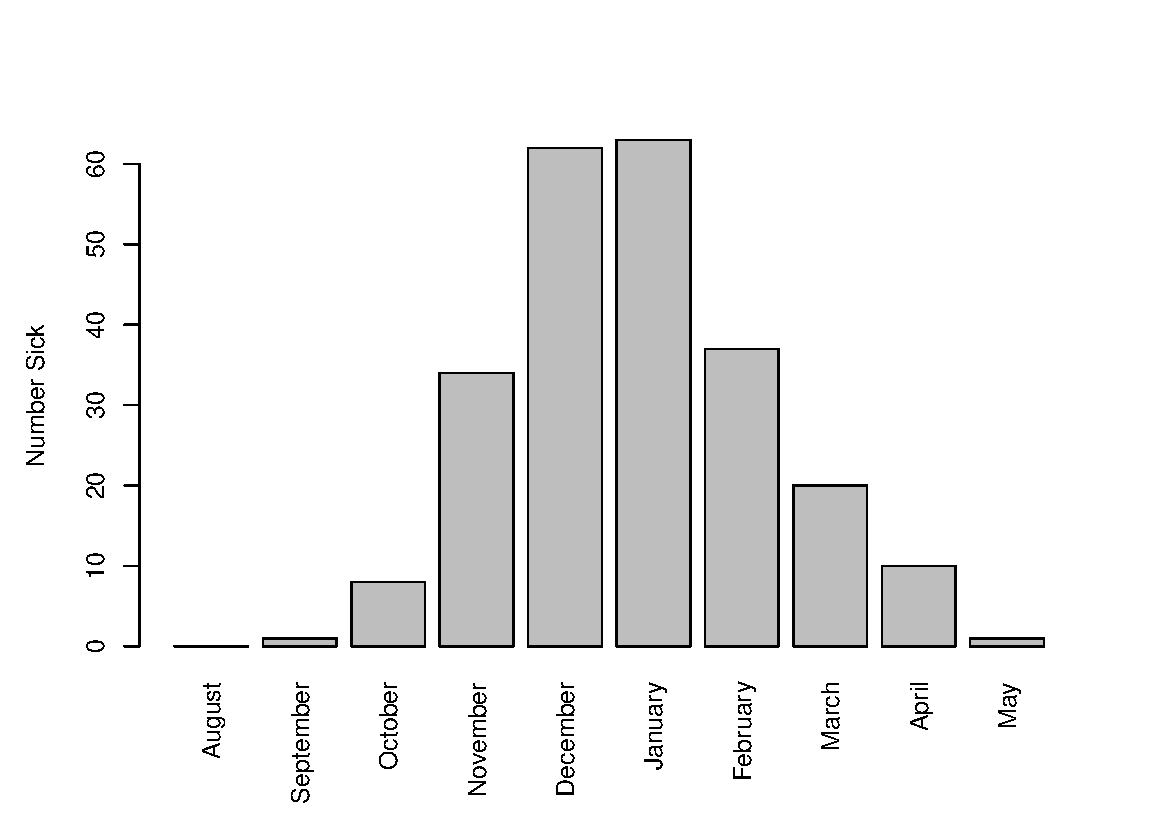
\includegraphics[width=.45\textwidth]{figs/sick_count.eps}
\caption{The rate of professionally diagnosed Influenza cases during the 2012-2013 season in our sample.}
\label{fig:flu_rate}
\end{figure}

\subsection{Twitter records}
While we received a total of 119 Twitter accounts, 15 were discarded because the associated accounts were either non-existent, banned, or private. For each of the remaining 104 accounts, we pulled their profile information, their friends and followers information, their most recent 3000 tweets, and their friends profiles and tweets. Some users did not tweet during the month that they were sick; we kept those accounts as part of the control group. We were limited to the most recent 3000 tweets by Twitter's time line query, but this only effected two accounts -- both of which posted multiple times per hour and were thrown out because we could only look back a few days.

We collected data by calling the Twitter API on the user account that we queried the longest time ago. Tweets, profile and follower information queries have separate rate limits and were collected in parallel. The 104 seed accounts collected above were given higher priority over their friends and followers. In total, we collected 37,599 tweets from the seed accounts and 30,950,958 tweets from 913,082 accounts that they either followed or were followed by.

%select count(distinct(d_net.user)) from (select distinct(user) as user from tweets_network) as d_net left join tweets on d_net.user = tweets.user where tweets.user is null;

%\section{Signal Detection}
\section{Text Based Signals}
\label{sec:text_analysis}

In this section, we consider diagnosis based on classifying an individual tweet's content as either about ILI or not. We begin by dividing the tweets into two sets: tweets that were posted the same month that a user was sick, and tweets that were posted other times. We find a total of 1609 tweets from 35 users in the first category.

First we go the route of defining a set of keywords that are positive signals of influenza. We chose \{flu, influenza, sick, cough, cold, medicine, fever\} as our set of keywords. Of these seven keywords, we find a significant effect in 6 of the keywords during months when the user had ILI. (See table \ref{tab:tweet_keyword_expert_results}). Additionally, we try algorithmically selecting keywords by first finding the 12,393 most common keywords in the data set.  We then rank them based off of information gain and choose the top 10, 100 or 1000 keywords from the list. In both of these cases, we preprocess the data by tokenizing the text on the characters ``.,;':"()?!'' - as well as spaces, tabs and line breaks - remove stop words\footnote{Stop words taken from Weka's stoplist version 3.7.10.}, perform Porter stemming \cite{Porter:1980dd,Willett:2006vb}  and convert the text to lower case. We then use the occurance or absence of these keywords as features for classification. We use naive bayes, random forest, J48, logistic regression and support vector machines to classify a user as being sick in a given month or not (see figure \ref{fig:roc_keyword}).



\begin{figure} [h]
\centering
\begin{subfigure}[b]{.2\textwidth}
\includegraphics[width=\textwidth]{figs/key_exp_roc.eps}
\end{subfigure}
\begin{subfigure}[b]{.2\textwidth}
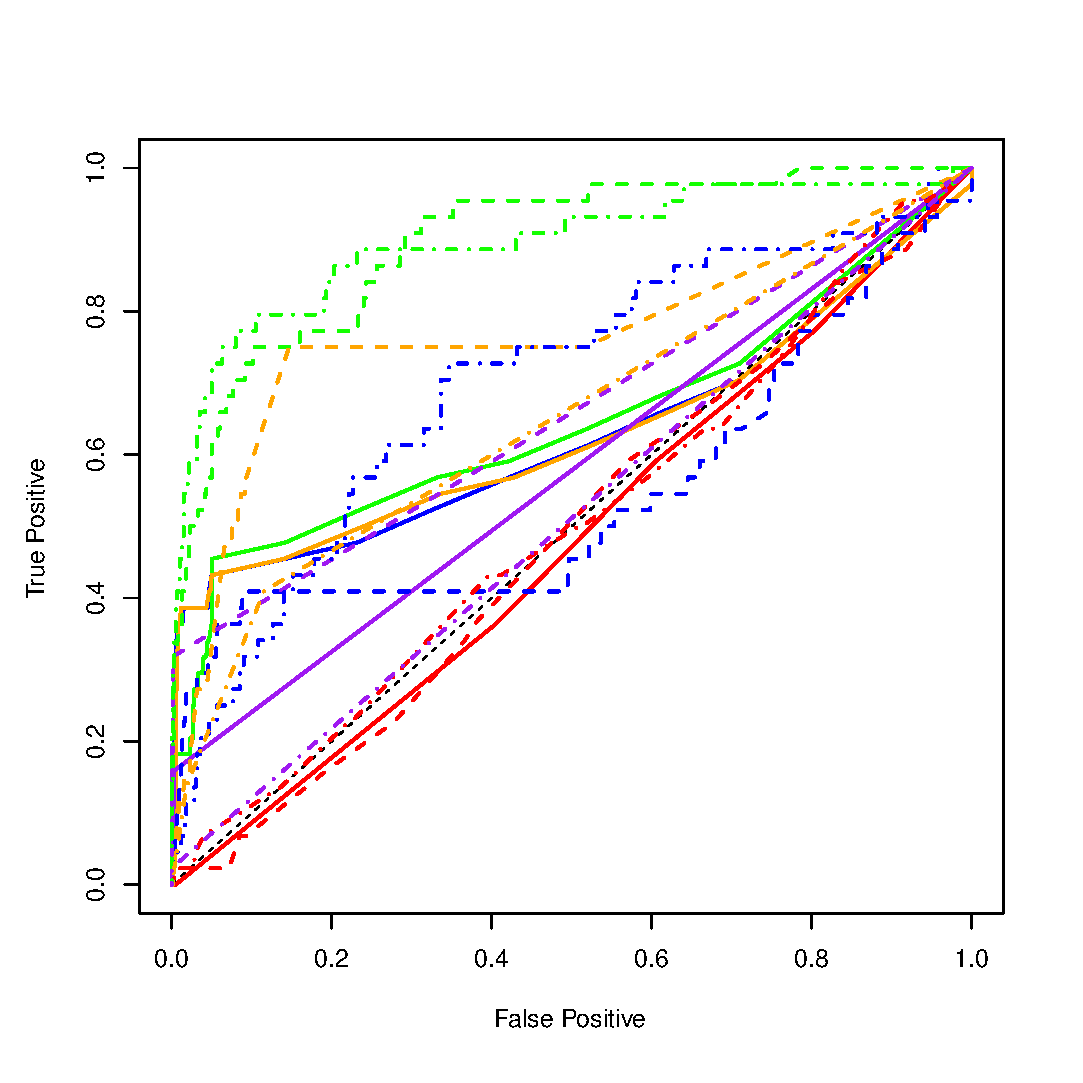
\includegraphics[width=\textwidth]{figs/key_dm_roc.eps}
\end{subfigure}
\begin{subfigure}[b]{.45\textwidth}
\includegraphics[width=\textwidth]{figs/keyword_legend.eps}
\end{subfigure}
\caption{The ROC of classifiers that use hand chosen keywords (a) and algorithmically chosen keywords (b) to determine if an individual is ill. The top 10 (solid line), 100 (dashed line) and 1000 (dotted line) were selected as the features.}
\label{fig:roc_keyword}
\end{figure}


Additionally, we hand rate all 1609 tweets, that were posted by individuals during the time of their illness,  for information regarding the user's health.  We also sample a randomly selected set of 1609 tweets from times when the users did not have ILI as a control. We find 58 tweets from 17 (\(17/35 = 48.57\%\))  individuals in our study that are about the user being sick. We also find zero tweets about ILI during times when they did \textit{not} have ILI. While the use of a ``human'' classifier clearly does not scale, it allows for an approxamatly 100.0\% accurate classification. Since regular machine learning algorithms preform much worse than 100.0\% accuracy, the human classifier gives us an upper limit to the accuracy of  a health monitoring system based off of tweet classification . (See table \ref{tab:tweet_classified_confusion})


%flu&25&40.14& \textless 0.0001 \ \\ \hline 
influenza&1&0.00&0.8325\ \\ \hline 
sick&128&5.22& \textless 0.0001 \ \\ \hline 
cough&18&4.48&0.0094\ \\ \hline 
cold&82&1.45&0.4154\ \\ \hline 
medicin&9&11.20& \textless 0.0001 \ \\ \hline 
fever&13&26.20& \textless 0.0001 \ \\ \hline 


\begin{table}
\centering
\begin{tabular}{|c|c|c|c|} \hline
Word& Total &Odds Ratio & Significance\ \\ \hline
flu&25&40.14& \textless 0.0001 \ \\ \hline 
influenza&1&0.00&0.8325\ \\ \hline 
sick&128&5.22& \textless 0.0001 \ \\ \hline 
cough&18&4.48&0.0094\ \\ \hline 
cold&82&1.45&0.4154\ \\ \hline 
medicin&9&11.20& \textless 0.0001 \ \\ \hline 
fever&13&26.20& \textless 0.0001 \ \\ \hline 

\end{tabular}
\caption{Keyword effects.}
\label{tab:tweet_keyword_expert_results}
\end{table}


\begin{table}
\centering
\begin{tabular}{|c|c|c|} \hline
Sick&Not Sick&\ \\ \hline
17 & 18 & Sick\\ \hline
0 & 66  & Not Sick\\
\hline\end{tabular}
\caption{Confusion matrix of a Tweet-Classification based diagnosis system. Rows are of true values, columns are of predicted values.}
\label{tab:tweet_classified_confusion}
\end{table}

\section{Frequency Based Signals}

It is likely that a user tweets at a different rate when she is ill than she normally does. To detect this, we perform one-dimensional anomaly detection on each user's monthly tweeting rate as follows. First, we calculate the number of tweets in each month in the study period and discard any months where the user tweets less than ten times. This avoids issues caused by the user starting or stopping to use Twitter. We then calculate the z-score of the tweeting rate of the month that the user is ill by

\begin{equation}
z = \frac{|x - \bar{x}|}{\hat{s}}
\end{equation}

Where \(\bar{x}\) and \(\hat{s}\) are the estimated mean and standard deviation of the user's tweeting rate. \cite{Grubs:1969ab} We repeat this process for months when the user is not sick. We then decide that the user is sick if \(z > 1.411\) where \(1.411\) was chosen through leave one out cross validation. We find a significant difference between the z-scores for months when a user was had ILI and months when the user did not (\(p = 0.01303\), two-sample Kolmogorov-Smirnov test). Most of the time individuals are not sick (219 / 258 = 84.88\%), resulting in a highly biased sample. Thus we optimize based on the \(F_1\) score instead of accuracy. The optimal z-score cutoff results in \(F_1= 35.0\%\). (See table \ref{tab:tweet_anomaly_confusion}.) 

%\begin{figure} %need to redo
%\centering
%\includegraphics[width=0.5\textwidth]{figs/meanFrequencies.eps}
%\caption{The frequency of tweeting behaviour of individuals in the months before, during and after an illness. Users significantly (check) decrease their rate of tweeting during the time that they had influenza. Dashed lines indicate the mean rate for the three months before / after the illness. (Todo: check significance)}
%\label{fig:mean_freq}
%\end{figure}

\begin{table}
\centering
\begin{tabular}{|c|c|c|} \hline
Sick&Not Sick&\ \\ \hline
14 & 25 & Sick\\ \hline
27 & 192 & Not Sick\\
\hline\end{tabular}
\caption{Confusion matrix of the classifier based on anomalous tweeting rates. Rows are of true values, columns are of predicted values.}
\label{tab:tweet_anomaly_confusion}
\end{table}

\section{Network Based Signals}

Even if a user is not currently active at all on Twitter, her friends or followers may give clues to her health status. We consider all text that a user's friends or followers tweeted and perform simular keyword analysis as was applied to the user's tweets in section \ref{sec:text_analysis}. Because the number and activity of friends or followers greatly varies regardless of a user's health status, we normalize the counts here by the total number of characters her friends or followers tweeted. We find that most of the tested classifiers are able to detect a signal in both the user's followers' and friends' streams. (See figure \ref{fig:roc_network}.)

%follower 12393
%friend 11595
%best = nb_1000 roc=.8641
\begin{figure} [h]
\centering
\begin{subfigure}[b]{.2\textwidth}
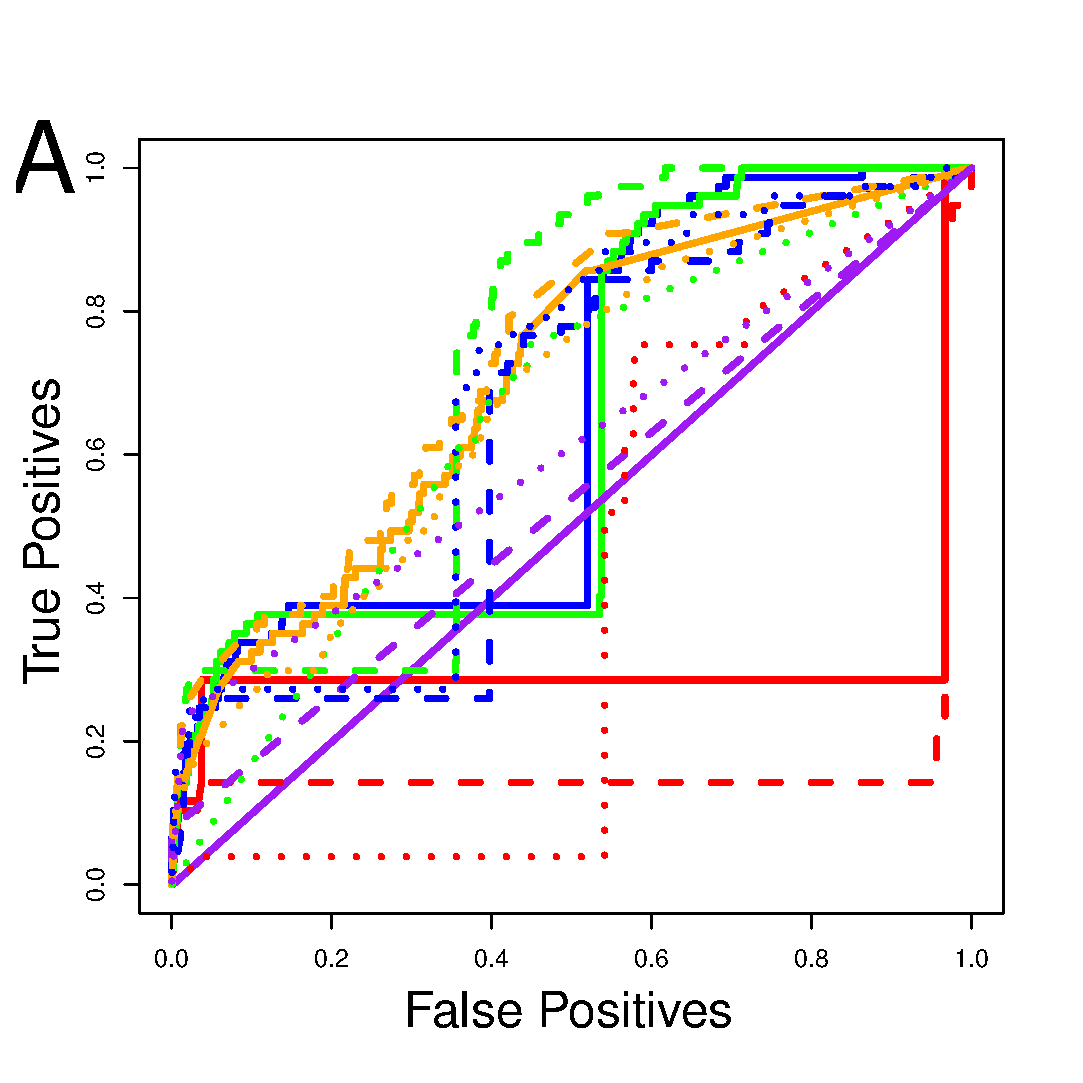
\includegraphics[width=\textwidth]{figs/followers_roc.eps}
\end{subfigure}
\begin{subfigure}[b]{.2\textwidth}
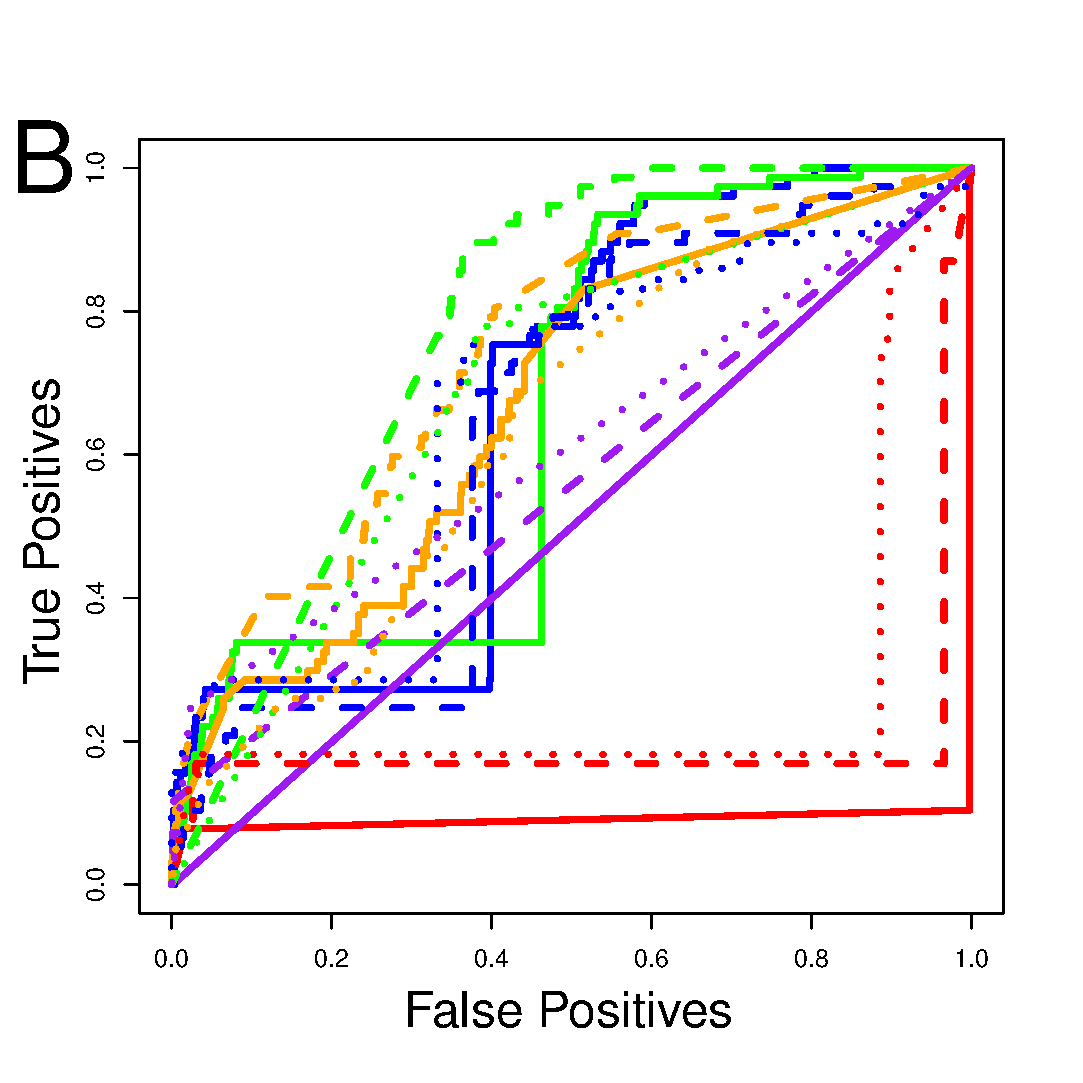
\includegraphics[width=\textwidth]{figs/friends_roc.eps}
\end{subfigure}
\begin{subfigure}[b]{.45\textwidth}
\includegraphics[width=\textwidth]{figs/keyword_legend.eps}
\end{subfigure}
\caption{The ROC of classifiers based off Tweets from (a) accounts that follow a user and (b) accounts that a user follows. Line coloring and style are equivalent to figure \ref{fig:roc_keyword}.}
\label{fig:roc_network}
\end{figure}

\section{Meta Classifier}

So far we have considered five seperate methods for detecting illness based off of a user's Twitter activity. However, there is no reason that we cannot combine these methods to get a stronger signal. For example, while mining the user's text is the best of the five methods, she may stop tweeting while sick, which would be detected by the frequency-based anomaly classifier. Aggregating multiple classifiers by a `meta-classifier' has been shown to be an effective method for increasing classification accuracy. \cite{Frossyniotis:2004wx,Todorovski:2003hk}


We start by selecting the classifier from each of the previous five approaches that has the largest area under the ROC curve (see figure \ref{fig:roc_meta} A). We then use the predicted distributions from these classifiers as the feature vector for the meta classifier. We use AdaBoost, bayesian classification, J48 decision trees, logit boost, and weighted voting to evaluate the meta-dataset. We then evaluate these methods with leave-one-out cross validation and see an increase in ROC area (and accuracy) over the best individual classifier (see figure \ref{fig:roc_meta} B).

%adaboost, weighted voting, logistic, j48 decision trees, basian model, stacking, logit boost

\begin{figure} [h]
\centering
\begin{subfigure}[b]{.2\textwidth}
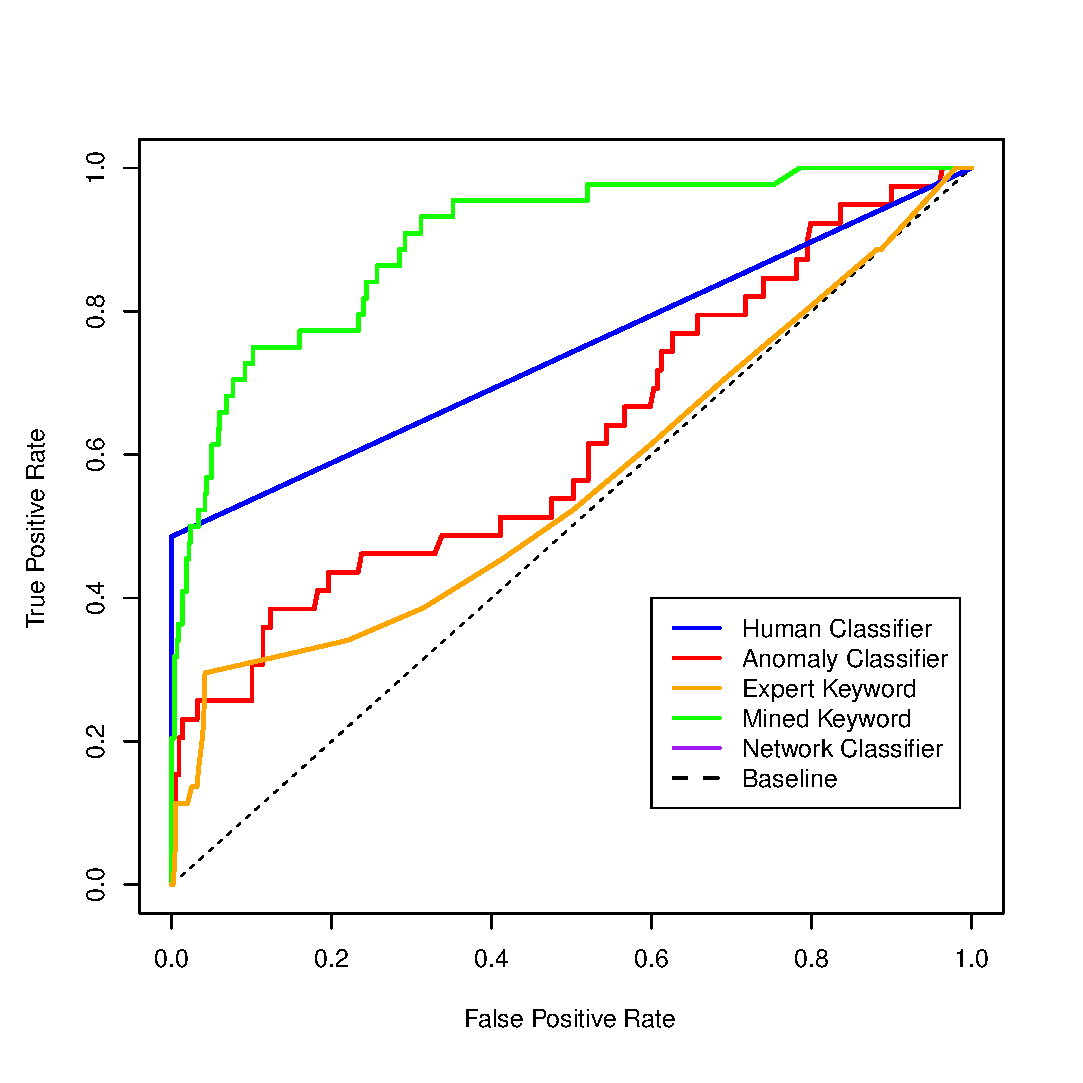
\includegraphics[width=\textwidth]{figs/meta_roc.eps}
\end{subfigure}
\begin{subfigure}[b]{.2\textwidth}
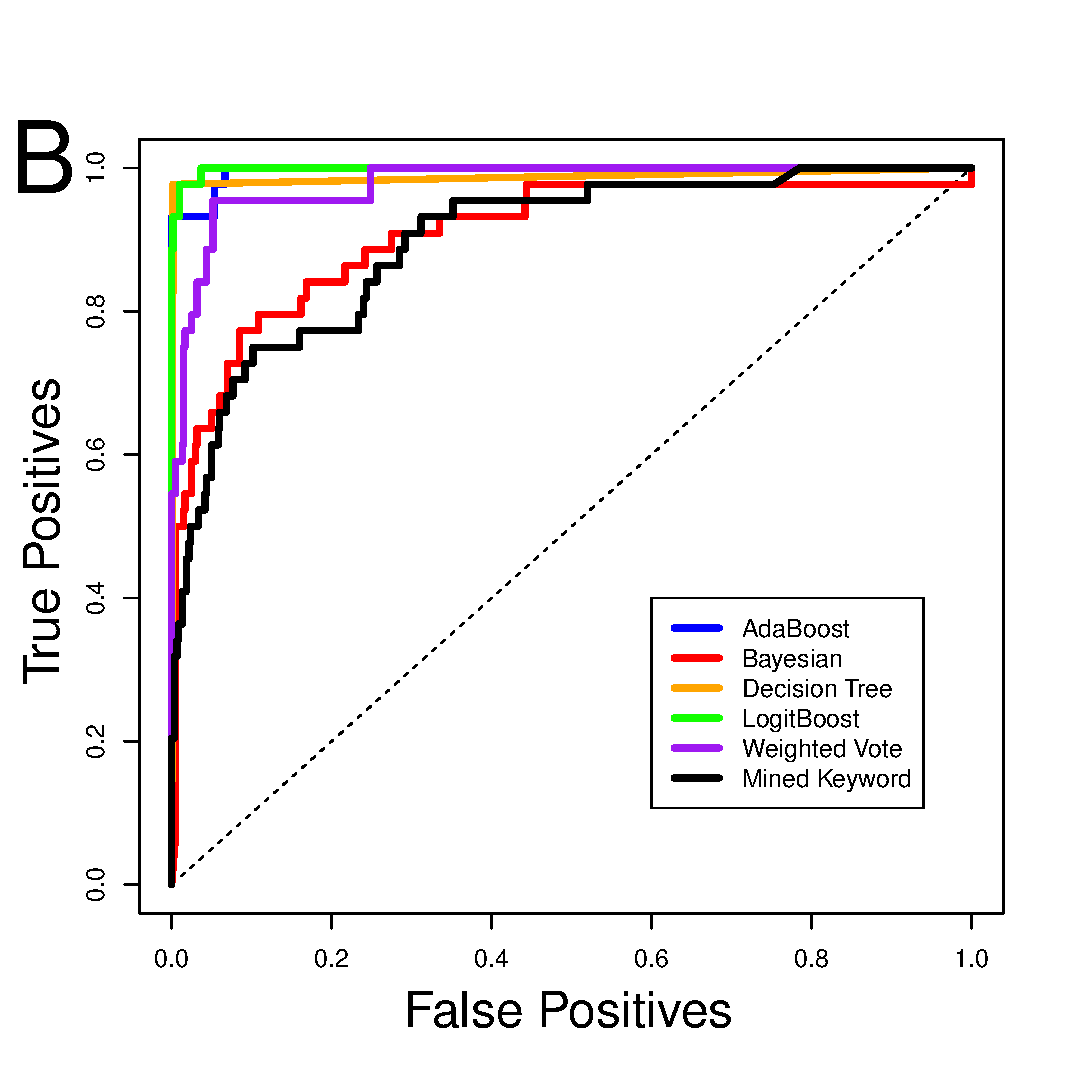
\includegraphics[width=\textwidth]{figs/meta_roc_final.eps}
\end{subfigure}
\caption{The accuracy of the previous classifiers (a) and the accuracy of various classifiers that use the previous classifier's results as features (b). }
\label{fig:roc_meta}
\end{figure}


\section{Conclusions}


In this paper, we have shown that it is possible to diagnose an individual based off of her social media data with high accuracy. Computational approaches to aid in disease diagnosis has been approached before, however they have been developed with a medical setting in mind. That is, the problem addressed was ``can we diagnose an individual based off data gathered from medical tests run on her?'' instead of ``can we diagnose an individual solely based off of publically available social media data?''  While we focus on the relativly benign case of remotely reconstructing a confidental diagnosis of Influenza, these methods could also be applied to stigmatized diseases, such as HIV, where being able to determine if an individual is HIV positive without her knowledge and with only her Twitter handle could result in serious social or economic effects. Half of the users explicitly stated that they were sick, and we were able to confidently determine illness in the other half of the cases through their data. It would seem that avoiding discussing a illness is not enough to hide one's health in the age of big data. 

%\section{Conclusions}

\section{Acknowledgments}

%\begin{thebibliography}{1}
%\bibitem{Ford:1956vc}
%L. R. Ford and D. R. Fulkerson. \newblock{Maximal Flow through a Network}. \newblock{\em Canadian Journal of Mathematics}, 8(3):399-404, 1956.
%\end{thebibliography}



%@article{Ford:1956vc,
%author = {Ford, L R and Fulkerson, D R},
%title = {{Maximal Flow through a Network.}},
%journal = {Canadian Journal of Mathematics},
%year = {1956},
%pages = {399--404}
%}


%
% The following two commands are all you need in the
% initial runs of your .tex file to
% produce the bibliography for the citations in your paper.
\bibliographystyle{abbrv}
\bibliography{library}  % sigproc.bib is the name of the Bibliography in this case
% You must have a proper ".bib" file
%  and remember to run:
% latex bibtex latex latex
% to resolve all references
%
% ACM needs 'a single self-contained file'!
%
%APPENDICES are optional
%\balancecolumns

\appendix
\ 


\begin{table}[!ht]
\centering
\begin{tabular}{|c|c|}\hline
Keyword&Ratio\ \\ \hline
flu &  34.424\\ \hline
health &  11.360\\ \hline
sick &  5.019\\ \hline
track & 10.952 \\ \hline
stud & 3.508 \\ \hline
asshol & 9.090 \\ \hline
ton & 9.090 \\ \hline
particip & 20.667 \\ \hline
salt & 20.667 \\ \hline
recov & 40.118 \\ \hline
fuck & 2.963 \\ \hline
sham & 13.64 \\ \hline
row & 10.180 \\ \hline
win & 2.947 \\ \hline
rt & 3.077 \\ \hline
  \end{tabular}
  \hspace{1em}
\begin{tabular}{|c|c|}\hline
cont. & \\ \hline
walk & 3.077 \\ \hline
childr & 6.820 \\ \hline
incred & 6.820 \\ \hline
meal & 6.820 \\ \hline
longer &  6.820 \\ \hline
succes &  26.765 \\ \hline
accis & 26.765 \\ \hline
holida & 26.765 \\ \hline
luv & 26.765 \\ \hline
oblig & 26.765 \\ \hline
path & 26.764 \\ \hline
pract & 26.764 \\ \hline
prayer & 26.765 \\ \hline
reserv & 26.765 \\ \hline
riot & 26.765 \\ 
\hline\end{tabular}
\caption{The thirty keyword stems with the highest positive predictive power ranked by significance. Ratio is calculated as the rate of occurance when a user is sick over the rate when a user is not sick.}
\label{tab:thirty_best}
\end{table}

\section{Keyword recomendations}


While our system should be trusted more than one based simply off of aggregated tweets, it is more computationally intensive than simply pulling data from a keyword stream. These systems require the user to select a specific set of keywords before data collection can begin. Keywords representing symptoms such as ``flu'', ``cough'', ``sore throat'', and ``headache'' are often chosen. We suggest that the thirty\footnote{The Twitter API limits queries to thirty keywords.} keywords with the highest postivie predictive value (see table \ref{tab:thirty_best}) be chosen as the parameters for a keyword stream. In addition to keywords related to symptoms (e.g. ``flu'' or ``sick'') we also find keywords related to treatments (e.g. ``health,'' ``prayer'' or ``recovery'') and keywords related to negative mood (e.g. vulgarities) to be more commonly tweeted when a user is ill. 


\balancecolumns

% That's all folks!
\end{document}
